\chapter{Framework Application for Design}
\label{chapter:application}

To verify that the conceptual framework is effective, I applied it to design a place photo discovery application. This chapter outlines the role the framework played in the design process of the Web application, the resulting application and its features, and some prospects for future application development. 

{\section{Applying the Conceptual Framework to Design an Application}
A need for a place photo discovery application was revealed during the construction phase of the framework. Asking questions from the preliminary framework (see Chapter~\ref{chapter:old_framework}) about existing applications, such as Pinterest and Google Maps, helped expose the need for discovery and curation of place photos with additional access to place location data and other details. It also helped gather some of the requirements for a photo discovery application.

In general, Web applications that are tailored towards image discovery, such as Pinterest and We Heart It, support user's motive to close a knowledge gap that is characterized by underdefined information need. To deal with the issue of having an underdefined information need, an application has to help the user to formulate their information need as well as support serendipitous discovery of information. In order to enable serendipitous discovery, Web applications regularly update the content they provide by allowing users to add new resources and curate information. 

The task of image seeking for the purpose of finding inspiration (as it is the case for the majority of Pinterest users) can stretch out to multiple sessions over an undetermined period of time. Curation mechanisms, such as preservation and management, help rediscover information to reflect on the previous findings and continue the task.  

It is common for users to discover place photographs on Pinterest, and Pinterest does display a map when a location of a place is known within the system. However, this feature only applies to a relatively small fraction of existing `pins'. In addition, Pinterest facilitates discovery of images related to diverse topics and interests, and not only places, which makes it harder to tailor user experience to facilitate discovery and curation based on the desired motives. 

When it comes to place discovery, the Google Maps application provides the ultimate support for finding place and business locations. It is also possible to see what a place looks like based on associated image. However, since the application is oriented towards finding specific information, visual and spatial photo exploration mechanisms are not well-developed. The user can preserve a given place but cannot preserve or organize photographs of places. Google Maps also lacks category-based navigation mechanisms which can help defining an information need.  

The findings above helped me define a motive for a place photo discovery application, which is to find inspirational (underdefined) place photographs, to collect and manage found information for future use and retrieval, as well as to provide access to more defined information about the place, such as its location. After formalizing the motive for the application use, I referred back to the framework to choose options for supporting various aspects of information discovery and curation while developing the application.
}

{\section{KeePlaces and Its Features}
The resulting application, KeePlaces\footnote[1]{A prototype of KeePlaces is available at www.keeplaces.com}, supports discovery and curation of place photographs, and it is integrated with Google Maps. This section outlines the main features of KeePlaces in accordance with the conceptual framework. 

Descriptional navigation is possible using search. The search feature is not guided, and so far, results are not personalized. 


Spatial exploration of multiple resources is enabled through the gallery view. 
Resources are represented as photos, so visual exploration of multiple resources is enabled. However, there is no way of exploring each resource individually, therefore, exploration of a single resource is not supported. 

KeePlaces is integrated with Google Maps.

Curation in Keeplaces is supported through management and preservation.

Management is implemented using collection-based classification.
Every photo discovered on the site can be bookmarked, or 'kept', in a collection.

Channeling has not yet been enabled within the application, but it is an important aspect behind the conceptual model of the application.


\begin{figure}[ht!]
	\noindent
	\centering
	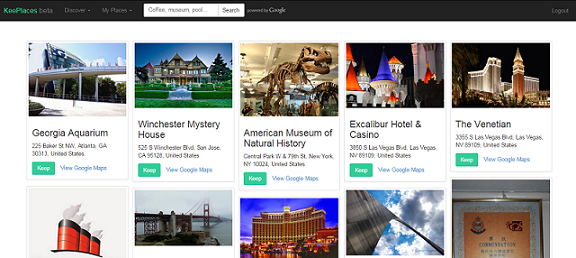
\includegraphics[width=\linewidth]{keeplaces.png}
	\caption{KeePlaces Interface}
	\label{fig:keeplaces} 
\end{figure}
}
{\section{Directions for Future Development}
As mentioned above, channeling is the first aspect that needs to be implemented along with enhancing management mechanisms.

} % end section

{\section{Discussion}


} % end section




